\documentclass[journal,12pt,twocolumn]{IEEEtran}
\usepackage[utf8]{inputenc}
\usepackage{amsmath}
\usepackage{mathtools}
\usepackage{txfonts}
\usepackage{listings}
\usepackage[define-L-C-R]{nicematrix}
\usepackage{hyperref}
\usepackage{multirow}

\renewcommand\thesection{\arabic{section}}
\renewcommand\thesubsection{\thesection.\arabic{subsection}}
\renewcommand\thesubsubsection{\thesubsection.\arabic{subsubsection}}

\renewcommand\thesectiondis{\arabic{section}}
\renewcommand\thesubsectiondis{\thesectiondis.\arabic{subsection}}
\renewcommand\thesubsubsectiondis{\thesubsectiondis.\arabic{subsubsection}}

\lstset{
%language=C,
frame=single,
breaklines=true,
columns=fullflexible
}

\def\putbox#1#2#3{\makebox[0in][l]{\makebox[#1][l]{}\raisebox{\baselineskip}[0in][0in]{\raisebox{#2}[0in][0in]{#3}}}}
     \def\rightbox#1{\makebox[0in][r]{#1}}
     \def\centbox#1{\makebox[0in]{#1}}
     \def\topbox#1{\raisebox{-\baselineskip}[0in][0in]{#1}}
     \def\midbox#1{\raisebox{-0.5\baselineskip}[0in][0in]{#1}}
\vspace{3cm}

\title{ASSIGNMENT 5}
\author{Anjana V\\AI20MTECH14010 }

\begin{document}
\numberwithin{equation}{subsection}
\newcommand{\myvec}[1]{\ensuremath{\begin{pmatrix}#1\end{pmatrix}}}
\newcommand{\mydet}[1]{\ensuremath{\begin{vNiceMatrix}[small]#1\end{vNiceMatrix}}}
\renewcommand{\vec}[1]{\mathbf{#1}}
\newcommand{\BAR}{%
  \hspace{-\arraycolsep}%
  \strut\vrule % the `\vrule` is as high and deep as a strut
  \hspace{-\arraycolsep}%
}
\maketitle
\begin{abstract}
This document aims to plot equation of circle with given points using matrices
\end{abstract}
Download all python codes from
%
\begin{lstlisting}
https://github.com/anjanavasudevan/grad_schoolwork/tree/master/EE5609/Assignment5/Code
\end{lstlisting}
%
and latex-tikz codes from
%
\begin{lstlisting}
https://github.com/anjanavasudevan/grad_schoolwork/tree/master/EE5609/Assignment5/Latex
\end{lstlisting}
%
\section{Question}
Find the equation to the circle that passes through the points:
\begin{align}
\vec{x_1} = \myvec{1\\2},\vec{x_2} = \myvec{3\\-4} , \vec{x_3} = \myvec{5\\-6}
\end{align}

\section{Answer}
The equation of circle in vector form is given by:
\begin{align}
\vec{x^Tx}+2\vec{x^Tu}+f = 0 \label{eq:1}
\end{align}
Using $\vec{x_1}, \vec{x_2}, \vec{x_3}$ in \eqref{eq:1},
\begin{align}
\vec{x_1}^T\vec{x_1}+2\vec{x_1}^T\vec{u}+f=0\\
\vec{x_2}^T\vec{x_2}+2\vec{x_2}^T\vec{u}+f=0\\
\vec{x_3}^T\vec{x_3}+2\vec{x_3}^T\vec{u}+f=0
\end{align}
The above system can be written in matrix form as:
\begin{align}
\myvec{2\vec{x_1}^T & 1\\2\vec{x_2}^T & 1\\2\vec{x_3}^T & 1}\myvec{\vec{u}\\f}=\myvec{-\vec{x_1}^T\vec{x_1}\\-\vec{x_1}^T\vec{x_1}\\-\vec{x_3}^T\vec{x_3}} \label{eq:2}
\end{align}
Substituting the values for $\vec{x_1}, \vec{x_2}, \vec{x_3}$ in \eqref{eq:2},
\begin{align}
\myvec{2 & 4 & 1\\6 & -8 & 1\\10 & -12 & 1}\myvec{\vec{u}\\f}&=\myvec{-5\\-25\\-61} \label{eq:3}
\end{align}
Using row echelon form to reduce \eqref{eq:3}, we get:
\begin{align}
\xleftrightarrow[R_3\rightarrow R_3-5R_1]{R_2\rightarrow R_2-3R_1}\myvec{2 & 4 & 1 &\BAR & -5\\0 & -20 & -2 &\BAR & -10\\ 0 & -32 & -4 &\BAR & -36}\\
\xleftrightarrow[R_3\rightarrow -\frac{1}{4}R_3]{R_2 \rightarrow -\frac{1}{2}R_2}\myvec{2 & 4 & 1 &\BAR & -5\\0 & 10 & 1 &\BAR & 5\\ 0 & 8 & 1 &\BAR & 9}\\
\xleftrightarrow[]{R_3 \rightarrow 5R_3-4R_2}\myvec{2 & 4 & 1 &\BAR & -5\\0 & 10 & 1 &\BAR & 5\\ 0 & 0 & 1 &\BAR & 25}\\ \label{eq:4}
\xleftrightarrow[R_2 \rightarrow \frac{1}{10}R_2]{R_1 \rightarrow \frac{1}{2}R_1}\myvec{1 & 2 & \frac{1}{2} &\BAR & -\frac{5}{2}\\[0.2cm]0 & 1 & \frac{1}{10} &\BAR & \frac{2}{5}\\[0.2cm] 0 & 0 & 1 &\BAR & 25}
\end{align}
Back solving the system using \eqref{eq:2} and \eqref{eq:4}, we get:
\begin{align}
\myvec{\vec{u}\\f}=\myvec{-11 \\ -2 \\ 25} \\
\implies \vec{u} = \myvec{-11 \\ -2}, f = 25
\end{align}
The equation of the circle that passes through the points $\vec{x_1}, \vec{x_2}, \vec{x_3}$ is given by:
\begin{align}
\vec{x^Tx}+2\myvec{-11 \\ -2}^T\vec{x}+f = 0 \\
\implies x^2 + y^2 - 22x -4y + 25 = 0
\end{align}
The plot of the circle is given below:
\begin{figure}[t]
\centering
    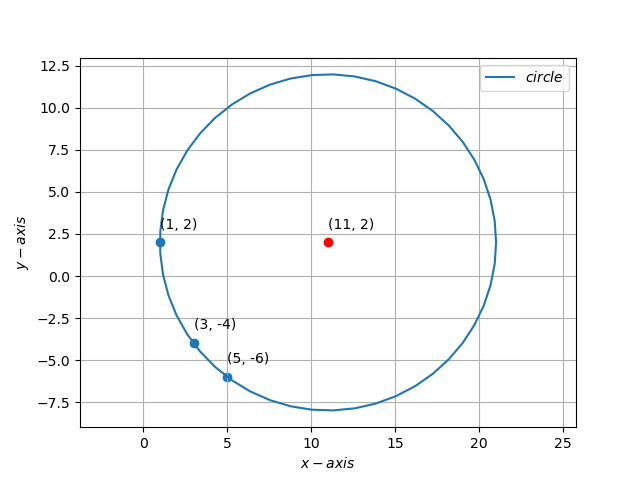
\includegraphics[width=\columnwidth]{Figure_1.png}
    \caption{Circle centered at $(11, 2)$ with radius $10$.}
    \label{fig:1}
\end{figure}
\end{document}
